\documentclass[11pt,a4paper]{article}
\usepackage[margin=2.2cm]{geometry}
\usepackage[T1]{fontenc}
\usepackage[utf8]{inputenc}
\usepackage{underscore}
\usepackage{graphicx}
\graphicspath{{../screenshots/}}
\usepackage{booktabs}
\usepackage{xcolor}
\usepackage{listings}
\usepackage{enumitem}
\usepackage{float}
\usepackage{caption}
\usepackage[colorlinks=true,linkcolor=blue!50!black,urlcolor=blue!60!black]{hyperref}

\lstset{
  basicstyle=\ttfamily\small,
  breaklines=true,
  frame=single,
  backgroundcolor=\color{gray!8},
  columns=fullflexible,
  keepspaces=true,
  xleftmargin=4pt,
  xrightmargin=4pt
}

\setlength{\parskip}{0.4em}
\setlength{\parindent}{0pt}

\title{\textbf{Kubernetes in Practice:\\ From Docker Compose to a Multi-Service Cluster}}
\author{Haroon (HaroonIMS)\\ Practice project, Peshawar, Pakistan}
\date{11 November 2026}

\begin{document}
\maketitle

\begin{abstract}
This report documents a hands-on practice project that follows a six-lab Kubernetes course. The work was done on a single laptop using kind (Kubernetes in Docker), with a three-node cluster, Traefik as the ingress controller, and a PostgreSQL database running inside the cluster. The project moved a Docker Compose application (a web site, a notes API, a tasks API, and a database) to Kubernetes, step by step, and tested how it behaves under failure, load, and change. Key results: rolling updates caused no client-visible errors once a readiness probe was added, and one error appeared before it; a release that crashed on start stalled the rollout when no readiness probe existed; a single ingress replica became a single point of failure during a node drain; and the tasks API scaled from 2 to 6 Pods at up to 792\% CPU before returning to 2. The application is published through a public HTTPS tunnel, and the manifests, source code, and screenshots are stored in a public GitHub repository.
\end{abstract}

\tableofcontents
\newpage

\section{Introduction}
Docker Compose runs an application on one machine. Kubernetes runs the same containers across a cluster and keeps them healthy, scaled, and updated without manual intervention. This project follows the course ``Kubernetes Fundamentals: From Compose to Kubernetes'' and applies each concept to a real application that was built earlier as a set of Docker labs.

The project had three goals:
\begin{enumerate}[leftmargin=*]
  \item Understand the core Kubernetes objects (Pods, Deployments, Services, Ingress, ConfigMaps, Secrets, StatefulSets, Jobs, and autoscalers) by using them.
  \item Test the behaviour the course promises: self-healing, data persistence, zero-downtime updates, rollback, autoscaling, and safe node maintenance.
  \item Publish the result as a reproducible project with documentation.
\end{enumerate}

\section{Environment and preparation}
\subsection{Machine and tools}
The project ran on an HP EliteBook 840 G5 with 8 CPUs and about 14 GB of RAM, running Ubuntu 24.04 in a dual-boot setup with Windows. The tool versions were:

\begin{table}[H]
\centering
\begin{tabular}{@{}ll@{}}
\toprule
Tool & Version \\
\midrule
Docker Engine & 29.1.3 (containerd image store) \\
kind & v0.34.0 \\
Kubernetes node image & v1.37.0 \\
kubectl & v1.37.2 \\
Helm & v3.22.1 \\
Traefik (chart 42.3.0) & v3.7.17 \\
metrics-server & v0.9.1 \\
PostgreSQL & 18.6 (postgres:18-alpine) \\
\bottomrule
\end{tabular}
\caption{Software used in the project.}
\end{table}

\subsection{Disk space problem}
The course requires about 20 GB of free disk space. At the start, the root partition had 2.9 GB free (91\% used). Most of the space was taken by a Multipass virtual machine (7.7 GB, a DevOps practice server that was left untouched), Docker and containerd image storage (about 3 GB), and system caches. Safe cleanup (pruning stopped containers and dangling images, clearing the apt cache, and trimming the system journal) freed only a few hundred megabytes.

The solution was to move Docker's storage to a larger partition. The steps were:
\begin{enumerate}[leftmargin=*]
  \item Add the partition to \texttt{/etc/fstab} with the \texttt{nofail} option, so it mounts at boot.
  \item Stop Docker and containerd, then copy \texttt{/var/lib/docker} (2.6 GB) and \texttt{/var/lib/containerd} (2.4 GB) with \texttt{rsync -aHAX}. The sizes matched on both sides.
  \item Rename the originals to \texttt{.old}, and create symbolic links at the original paths that point to the new partition.
  \item Start the services, then reboot to confirm everything returns automatically. It did.
  \item Delete the \texttt{.old} copies. The root disk went from 2.9 GB to 6.9 GB free, and the storage partition held the Docker data with 57 GB free.
\end{enumerate}

\subsection{Incident: data loss on a partition}
\textbf{This was an error, and it is recorded here so it is not repeated.} While preparing the partition, it was mounted to check its contents. It held an old Linux root filesystem. The partition was then formatted with \texttt{mkfs.ext4} after a confirmation prompt, which erased that data. The Windows partitions and the Linux root were not touched, and the copy of the project folder made earlier was kept. The lesson: before formatting any partition, identify its contents with \texttt{blkid} and back up anything needed.

\section{From Compose to Kubernetes}
The application had four services. Table~\ref{tab:mapping} shows how each one was rebuilt.

\begin{table}[H]
\centering
\small
\begin{tabular}{@{}p{4.2cm}p{5.8cm}p{4.2cm}@{}}
\toprule
Compose service & Kubernetes objects & File \\
\midrule
\texttt{.env} database passwords & Secret \texttt{db-credentials} (created with kubectl) & none (not stored) \\
\texttt{db} with \texttt{pgdata} volume & StatefulSet, headless Service, PVC template & \texttt{db.yaml} \\
\texttt{db} healthcheck & Readiness probe running \texttt{pg\_isready} & \texttt{db.yaml} \\
\texttt{notes} service & Deployment, Service, ConfigMap & \texttt{notes.yaml} \\
\texttt{tasks} service and \texttt{DATABASE\_URL} & Deployment, Service, environment built from the Secret & \texttt{tasks.yaml} \\
\texttt{migrate} service & Job that runs before the API starts & \texttt{migrate-job.yaml} \\
\texttt{depends\_on: service\_healthy} & Init container that waits for the database & \texttt{tasks.yaml} \\
\texttt{web} service & Deployment, Service, nginx ConfigMap & \texttt{web.yaml} \\
\texttt{proxy} with nginx config & Traefik, Ingress rules, strip-prefix Middleware & \texttt{ingress.yaml} \\
\texttt{restart: unless-stopped} & Controllers and probes & all files \\
\bottomrule
\end{tabular}
\caption{Mapping of the Compose application to Kubernetes.}
\label{tab:mapping}
\end{table}

\section{Laboratory work}

\subsection{Lab 1: Building and exploring the cluster}
\textbf{Goal.} Install the tools, create a three-node cluster, and inspect its control plane and worker nodes.

\textbf{Work.} The three tools were installed from official release binaries. The cluster was created from a configuration file with one control-plane node and two workers, with port mappings 8080 and 8443 for later use. Each Kubernetes node is a Docker container on the laptop, which is what makes a local cluster possible.

\begin{lstlisting}
kind create cluster --config kind-config.yaml
kubectl get nodes -o wide
kubectl get pods -n kube-system -o wide
kubectl describe node bootcamp-worker
\end{lstlisting}

\textbf{Results.} All three nodes were \texttt{Ready}, and all 12 system Pods were \texttt{Running}. The control-plane components (etcd, API server, scheduler, controller manager) ran only on the control-plane node. The networking components ran on every node.

\textbf{Observations.}
\begin{itemize}[leftmargin=*]
  \item Inspecting the API server manifest showed how its flags set identity, authorization (\texttt{Node,RBAC}), the etcd address, and the service IP range.
  \item Stopping a worker container made it \texttt{NotReady}. A stop of only a few seconds did not trigger the change, because the control plane waits for missed heartbeats before reacting.
  \item Deleting and recreating the cluster took 46.6 seconds.
\end{itemize}

\subsection{Lab 2: Release management}
\textbf{Goal.} Deploy the notes API with four replicas, upgrade it, break it on purpose, roll back, and observe a node failure.

\textbf{Setup.} The handbook's notes API is a Node.js application. The project used the Flask notes API from the earlier Docker labs, with a version route added so the course's version checks work. The application listens on port 5000, and the Service maps port 3000 to it, as the Ingress expects.

\textbf{Work and results.}
\begin{enumerate}[leftmargin=*]
  \item \textbf{First deployment (1.0.0).} Four Pods were spread across both workers, and the rollout completed.
  \item \textbf{Continuous calls through port-forward.} Every response came from one Pod, with version 1.0.0.
  \item \textbf{Rolling update to 1.1.0.} The rollout took about 25 seconds with no downtime. The snapshots showed the old ReplicaSet and the new one trading Pods, with at most five Pods at once (\texttt{maxSurge: 1}).
  \item \textbf{Broken image tag (9.9.9).} The new Pod stayed in \texttt{ErrImagePull} and then \texttt{ImagePullBackOff}. The four working Pods kept serving, because \texttt{maxUnavailable: 0} never removes a working Pod before its replacement is ready. A rollback restored the previous version.
  \item \textbf{Release that crashes on start.} The release printed no error during the rollout, but each new Pod ran for a few seconds, reported ready, and then crashed. Kubernetes counted it as available and removed the old Pods, so the Deployment had zero ready Pods for a period. The rollout timed out, and a rollback recovered the service. This failure is the reason readiness probes are required.
  \item \textbf{Node failure.} When the worker was stopped for about five minutes, its Pods were marked \texttt{Unknown}, and replacements were created on the other worker. The events showed the node \texttt{NotReady} at 7m35s before the query, and the replacement scheduled at 2m34s, a gap of 5 minutes 1 second. This matches the default eviction timeout. The replacement itself took about one second, because the image was already on that node.
\end{enumerate}

\subsection{Lab 3: Services and Ingress}
\textbf{Goal.} Expose several services behind one entry point, with path routing, middleware, HTTPS, and a load test through the Ingress.

\textbf{Work.} The \texttt{notes} and \texttt{web} Deployments received ClusterIP Services. Traefik was installed with Helm, exposed through NodePorts 30080 and 30443, which kind maps to the laptop's ports 8080 and 8443. The Ingress routed \texttt{/api/notes} to the notes Service and everything else to the web Service. A \texttt{replacePath} Middleware made \texttt{/notes-info} reach the notes root route. A self-signed certificate for \texttt{bootcamp.local} was stored as a TLS Secret, and it was tested with \texttt{curl --resolve}.

\textbf{Results.} The ingress answered with 404 at first, then with 200 after about ten seconds, as Traefik loaded the new rule. A zero-downtime test used a request loop of 0.2 seconds during a rolling update. The first rollout produced:

\begin{table}[H]
\centering
\begin{tabular}{@{}lrl@{}}
\toprule
HTTP status & Count & Interpretation \\
\midrule
200 & 37 & New version Pods \\
404 & 333 & Old version Pods, which had no route yet \\
502 & 1 & A request reached a Pod that was not listening yet \\
\bottomrule
\end{tabular}
\caption{First rolling update, without a readiness probe.}
\end{table}

A readiness probe on \texttt{/health} was then added. A second restart produced 196 responses, all \texttt{200}, which shows the probe kept traffic away from Pods that were not ready.

\textbf{Observation.} Two of the course's instructions needed adjustment. The Traefik values file had to place the service type at the top level, and the course's browser address (a VM IP) became \texttt{localhost:8080}, because the cluster runs on the laptop.

\subsection{Lab 4: A database that survives}
\textbf{Goal.} Run PostgreSQL in the cluster with durable storage, and prove that Pods and the StatefulSet can be deleted and recreated without losing data.

\textbf{Work.} The password was stored in a Secret, not in the YAML file. The StatefulSet created the Pod \texttt{db-0} and the claim \texttt{data-db-0}, bound to a 1~GB volume. A table with two rows was created.

\textbf{Results.}
\begin{itemize}[leftmargin=*]
  \item Deleting \texttt{db-0} recreated it under the same name. It reattached to the same claim, and the rows came back with identical timestamps.
  \item Deleting the StatefulSet left the claim \texttt{Bound}. Reapplying the manifest restored the database with the same data.
  \item A \texttt{pg\_dump} backup of 1.2~KB restored into a scratch database, with the expected \texttt{COPY 2} row count.
  \item The nightly backup CronJob, in its first version, failed silently. The \texttt{pg\_dump} command could not authenticate, because it reads \texttt{PGPASSWORD} rather than \texttt{POSTGRES\_PASSWORD}. The script's last command (an \texttt{echo}) succeeded, so Kubernetes reported success. The fix was \texttt{set -e} and an explicit \texttt{PGPASSWORD} export. The corrected job produced a 1169-byte backup.
\end{itemize}

\textbf{Observation.} The backup was written to a temporary location inside the Pod, so a real deployment must copy it to storage that outlives the job.

\subsection{Lab 5: Healthy and elastic}
\textbf{Goal.} Set resource requests and limits, add probes, install metrics, scale automatically, drain a node during traffic, and protect the application with a PodDisruptionBudget.

\textbf{Resources and probes.} Requests were 100m CPU and 64Mi memory, and limits were 500m CPU and 128Mi memory. A liveness probe on \texttt{/health} was added, which does not touch the database, so a database outage cannot restart the notes Pods. The Pods were classified as \texttt{Burstable}.

\textbf{Metrics.} metrics-server was installed. Node-level usage was between 1\% and 5\% of CPU and memory on all three nodes. The notes Pods used about 3 millicores and 26 to 29 MiB each. The kubelets used certificates that metrics-server could not verify, so the flag \texttt{--kubelet-insecure-tls} was added. This flag is only suitable for a local cluster.

\textbf{Autoscaling.} A HorizontalPodAutoscaler with a minimum of 2, a maximum of 6, and a 50\% CPU target was attached to the notes Deployment. The \texttt{replicas} field was removed from the Deployment so the autoscaler owns the count.

\begin{table}[H]
\centering
\begin{tabular}{@{}lrrl@{}}
\toprule
Event & CPU & Replicas & Time \\
\midrule
Idle, before load & 3\% & 2 & before 21:12 \\
Load started & 330\% & 2 & 21:12:06 \\
First scale-up step & 443\% & 4 & about 15 s later \\
Peak & 405\% & 6 & about 30 s later \\
Load removed & 3\% & 6 & 21:13:39 \\
Back to 2 replicas & 3\% & 2 & 21:19:46 \\
\bottomrule
\end{tabular}
\caption{Notes HPA during the load test. The scale-down took 6 minutes 7 seconds.}
\end{table}

\textbf{Drain under traffic.} With a request loop running through the Ingress, \texttt{bootcamp-worker} was cordoned and drained. The first drain moved no notes Pods, because the autoscaler had already moved them. It did move Traefik, which ran as a single replica. The loop recorded 73 responses with status 200 and 10 with status 000, which means no connection was possible for about two seconds. The application Pods were still serving; the single ingress replica was the failure point. In a second test, with Traefik on the other worker, 211 requests all returned 200.

\textbf{PodDisruptionBudget.} A budget with \texttt{minAvailable: 2} was applied. When one notes Pod was placed on the drained worker, the drain was blocked repeatedly with the message \texttt{Cannot evict pod as it would violate the pod's disruption budget}, and it timed out after 90 seconds. The Pod remained running. The budget protected availability at the cost of blocking maintenance.

\subsection{Lab 6: The capstone}
\textbf{Goal.} Deploy the complete application from one folder of manifests, verify it end to end, test its resilience, scale its services, publish it, and document it.

\textbf{Deployment.} The namespace was recreated, and the manifests were applied in this order: the database, then the migration Job, then the notes, tasks, and web Deployments, the Services, and the Ingress rules. The tasks API does not create its own table, so the Job runs first (a one-time Pod that creates the \texttt{tasks} table). The web site used the nginx stand-in with the handbook's ConfigMap. The overview command showed three Deployments at \texttt{2/2}, a StatefulSet at \texttt{1/1}, all Services and Ingresses, the bound claim, and Pods spread across both workers.

\textbf{Resilience tests.}
\begin{enumerate}[leftmargin=*]
  \item \textbf{Self-healing.} Both tasks Pods were deleted. Replacements reached \texttt{1/1} in about 13 seconds.
  \item \textbf{Data survival.} \texttt{db-0} was deleted and was back in about 3 seconds. The task created earlier was still in the list.
  \item \textbf{Readiness protects users.} The database was scaled to zero. The tasks Pods first returned errors from the application (HTTP 500), because the readiness probe checks the database only every five seconds and needs three failures. After the probe failed, the Pods showed \texttt{0/1} and requests returned 503 from Traefik. Scaling the database back up made the Pods ready again, without intervention.
  \item \textbf{Zero-downtime update.} A rolling restart of the notes Deployment ran while 163 requests were made. All returned 200.
  \item \textbf{Rollback.} An environment change created a new revision, and \texttt{kubectl rollout undo} restored the previous one. The running application read its setting from the ConfigMap, which confirmed the rollback.
\end{enumerate}

\textbf{Autoscaling of the tasks API.} A HorizontalPodAutoscaler with the same settings was attached to the tasks Deployment. The tasks API used much more CPU than notes per request, which is explained below. Under load on \texttt{/tasks}, CPU rose from 22\% to 634\% of the target within about two minutes. The HPA scaled 2 to 4 Pods at 792\% CPU, then to 6 at 664\%, and it stayed there while the load ran. After the load was removed at 02:20:58, the HPA waited, reduced the count to 3, and then to 2. The return to 2 replicas was confirmed at 02:32:49.

\textbf{Observation on CPU use.} Each tasks request opened a new PostgreSQL connection, which is expensive. A connection pool would reduce both CPU and the number of Pods needed.

\textbf{Public access.} The handbook serves the application through nginx on a VM with a domain. The project's network could not establish the quick tunnel (the request to the Cloudflare service timed out), so ngrok was used instead. It forwarded the public HTTPS address to Traefik on \texttt{localhost:8080}. An offline tunnel returned ngrok error ERR\_NGROK\_3200, and restarting the tunnel restored access. Figure~\ref{fig:ngrok} shows requests from the public address, each returning 200 OK, and Figure~\ref{fig:nginx} shows the web site in a browser over HTTPS.

\begin{figure}[H]
\centering
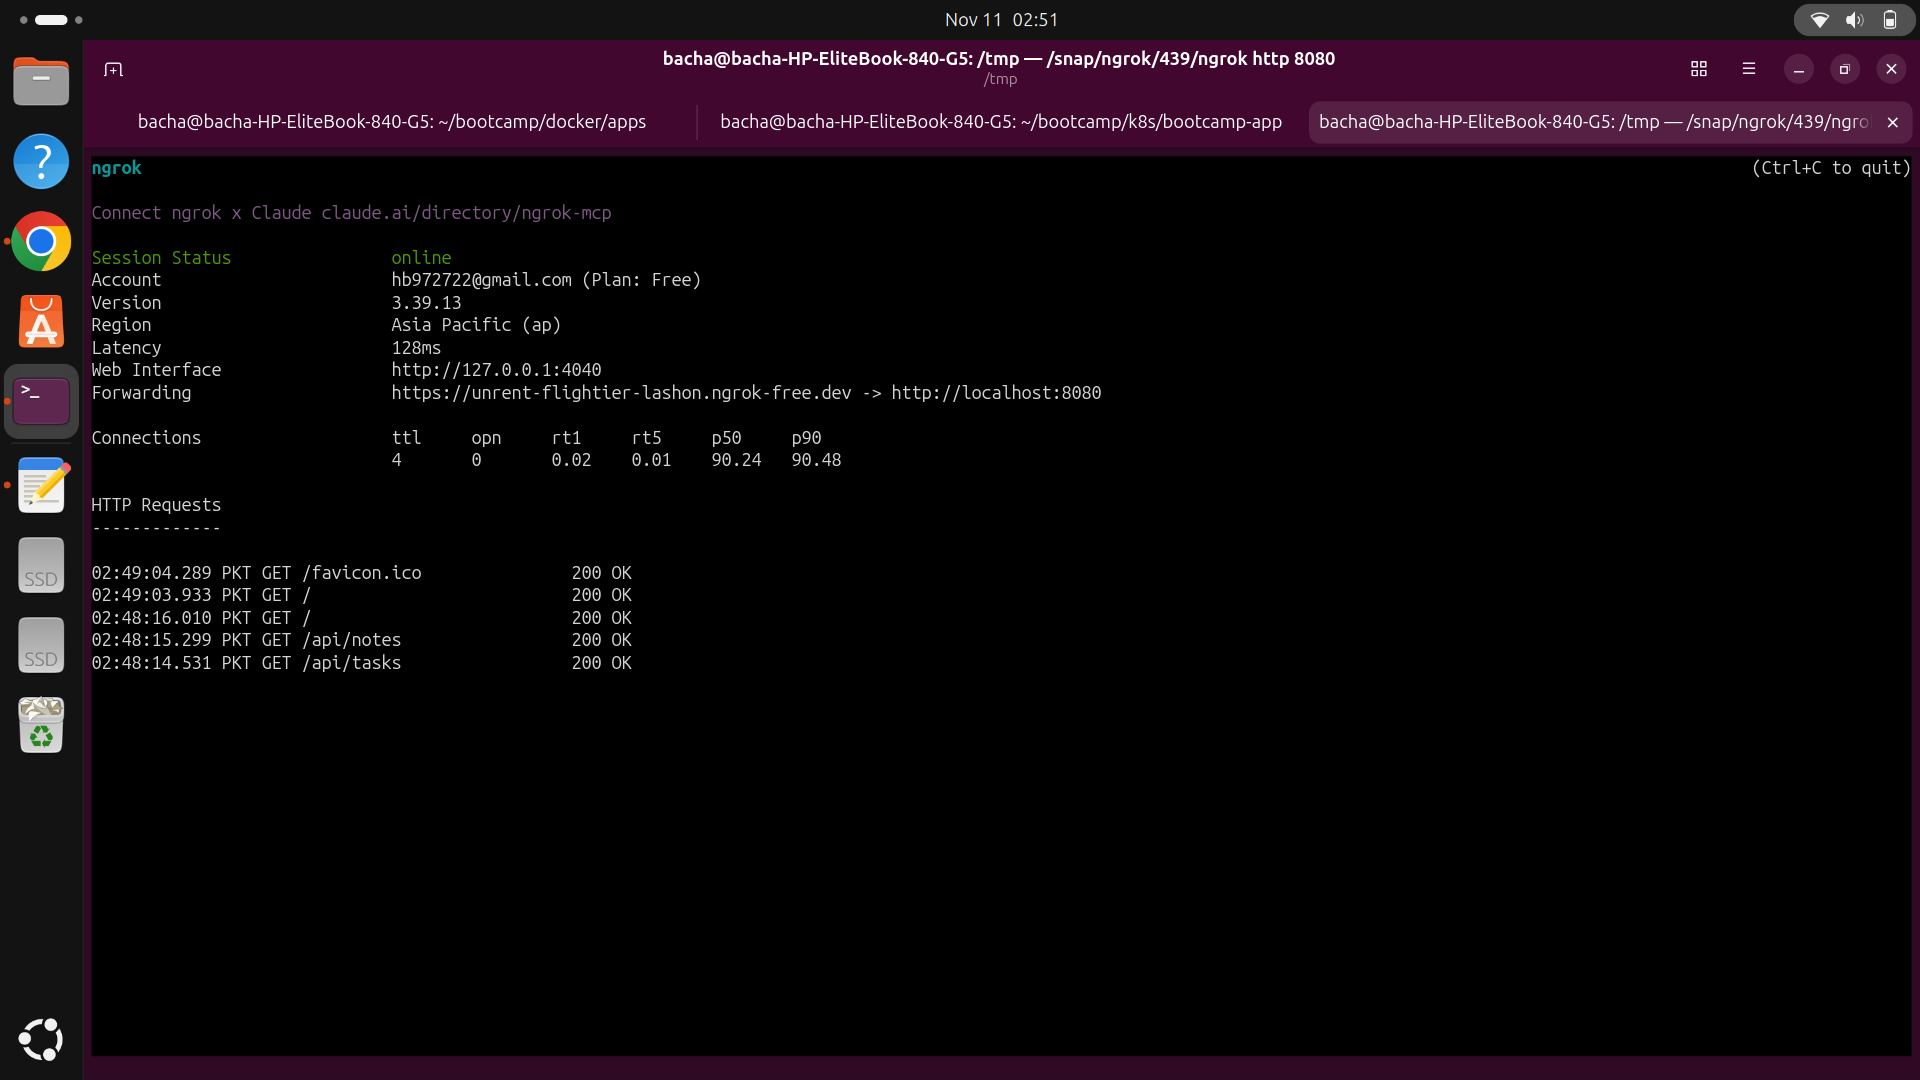
\includegraphics[width=\linewidth]{ngrok-requests.png}
\caption{Requests through the public ngrok address. \texttt{/api/tasks}, \texttt{/api/notes}, and \texttt{/} all returned 200 OK.}
\label{fig:ngrok}
\end{figure}

\begin{figure}[H]
\centering
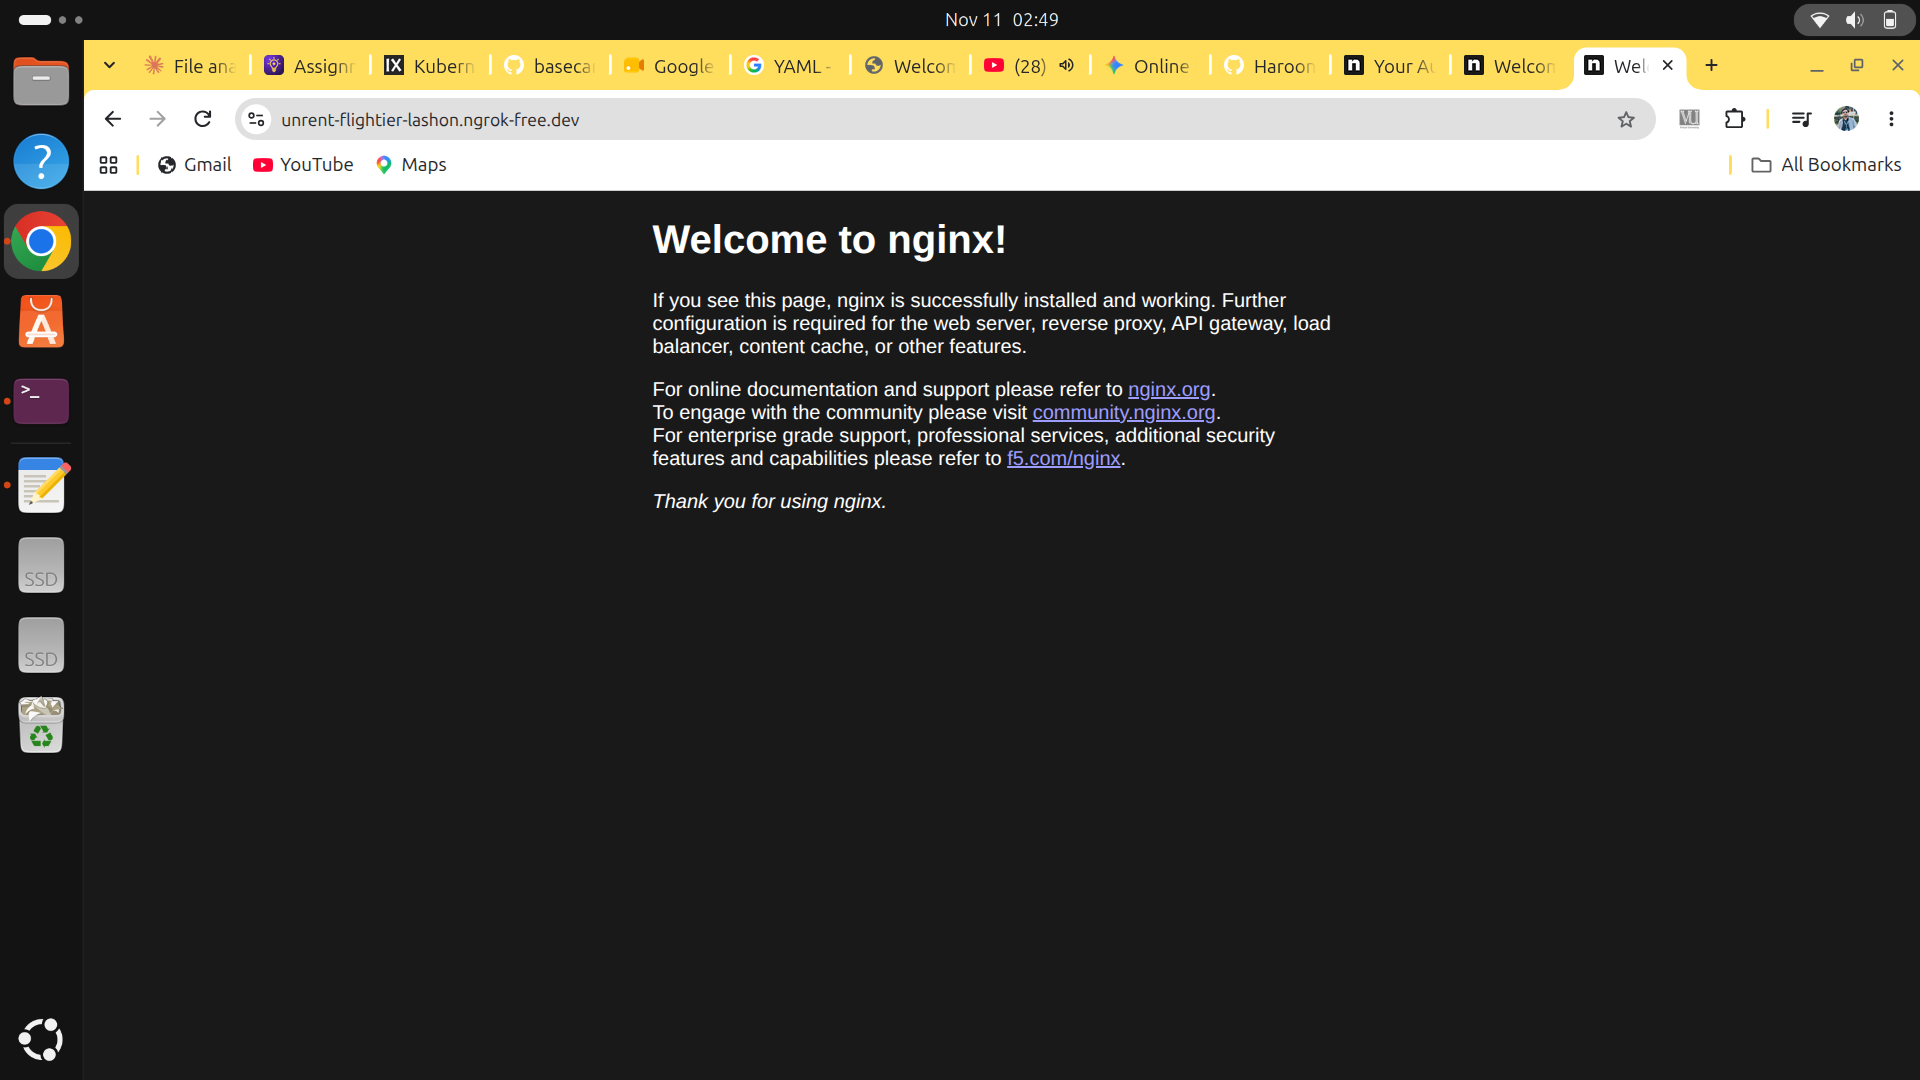
\includegraphics[width=0.85\linewidth]{nginx-welcome.png}
\caption{The web site served over HTTPS through the public address.}
\label{fig:nginx}
\end{figure}

\section{Deviations from the handbook}
\begin{table}[H]
\centering
\small
\begin{tabular}{@{}p{4.5cm}p{5.5cm}p{5.5cm}@{}}
\toprule
Area & Handbook & Project \\
\midrule
Notes API & Node.js, port 3000 & Flask, port 5000 (Service on 3000); version route and an in-memory \texttt{/api/notes} route added \\
Web site & React build, image \texttt{web:1.0.0} & \texttt{nginx:alpine} with the handbook's ConfigMap \\
Notes replicas & 3 in Lab 5, 2 in Part 12 & 4 in Labs 2 and 3, 2 in Part 12 \\
Traefik values & Service type under \texttt{spec} & Service type at the top level \\
Public URL & nginx on a VM with a domain & ngrok tunnel to the laptop \\
Ingress replicas & Not specified & One replica, which was a single point of failure \\
Database password & Chosen by the student & Development value, never stored in the repository \\
\bottomrule
\end{tabular}
\caption{Differences between the handbook and this project.}
\end{table}

\section{Problems encountered and lessons}
\begin{table}[H]
\centering
\small
\begin{tabular}{@{}p{4.3cm}p{5.3cm}p{5.4cm}@{}}
\toprule
Problem & Cause & Lesson \\
\midrule
Root disk at 91\% & Multipass VM and Docker images & Check sizes with \texttt{du} before cleaning; move data rather than delete \\
Partition data erased & Format run before identifying contents & Identify and back up before formatting \\
Certificate error on kubectl & Cluster created while the clock was wrong & Check \texttt{date} and NTP; rebuild the cluster \\
Namespace missing after rebuild & Rebuild removes all objects & Recreate the namespace and reload images after each rebuild \\
Silent backup failure & Script ended with a command that always succeeds & Use \texttt{set -e}; check the job status, not only the wait \\
Forbidden error after restart & API server still starting & Wait 10 to 30 seconds after restarts \\
502 during rolling update & No readiness probe & Add readiness probes before rolling updates \\
Crashing release stalls rollout & No readiness probe, so crashing Pods counted as ready & Readiness probe plus \texttt{progressDeadlineSeconds} \\
Drain blocks or evicts unexpectedly & Single ingress replica; budget with two replicas & Run ingress with two replicas and its own budget \\
Quick tunnel timeout & Network blocks the quick-tunnel service & Use a second provider \\
\bottomrule
\end{tabular}
\caption{Problems encountered during the project and what was learned.}
\end{table}

\section{Discussion}
\begin{enumerate}[leftmargin=*]
  \item \textbf{Rolling updates and readiness.} If a new version's readiness probe never passes, the rollout stalls with \texttt{maxUnavailable: 0}. Users keep the old, working version, which is good. But the release is incomplete until someone fixes or rolls back, so a progress deadline should be set to report the stall.
  \item \textbf{One entry point or one load balancer per service.} One ingress controller with path rules gives a single public address, one place for certificates, and one set of routes. The trade-off is that it becomes a shared dependency. A load balancer per service avoids that dependency but multiplies cost and configuration.
  \item \textbf{Running a customer database on Kubernetes.} Before doing so, a team should know who handles replication and failover, where backups are stored and how restores are tested, what recovery times are required, and who is on call. A managed database service or a database operator is often the safer choice.
  \item \textbf{Response format changes during a rolling update.} Old and new versions serve traffic at the same time, so a client can receive different formats from consecutive requests. Changes should add fields rather than rename or remove them.
\end{enumerate}

\section{Conclusion}
The project moved a three-service application from Docker Compose to a Kubernetes cluster and tested it under the conditions that matter in production: failures, updates, load, and maintenance. Several results were counterintuitive and became the most useful lessons. Zero downtime depends on readiness probes, not only on the rolling-update strategy. Scaling and maintenance work only when requests and budgets are set correctly. Single components that look minor, such as one ingress replica, can cause outages during routine work. The application is published through a public HTTPS address, and its code and documentation are in a public repository.

\subsection*{Resources}
\begin{itemize}[leftmargin=*]
  \item Repository: \url{https://github.com/HaroonIMS/bootcamp-k8s}
  \item Public address during the demonstration: \url{https://unrent-flightier-lashon.ngrok-free.dev}
\end{itemize}

\appendix
\section{Repository layout}
\begin{lstlisting}
bootcamp-k8s/
  README.md               deployment guide and deviations
  .gitignore              excludes secrets, certificates, and dumps
  kind-config.yaml        cluster definition
  traefik-values.yaml     ingress controller settings
  k8s/                    manifests: db, notes, tasks, web, ingress,
                          migrate-job, hpa
  notes-api-app/          Flask notes API source and Dockerfile
  tasks-api-app/          FastAPI tasks API source and Dockerfile
  docs/screenshots/       images used in the README and this report
  docs/report/            this report (LaTeX source and PDF)
\end{lstlisting}

\section{Deployment order}
\begin{lstlisting}
kubectl apply -f k8s/db.yaml
kubectl rollout status statefulset db
kubectl apply -f k8s/migrate-job.yaml
kubectl wait --for=condition=complete job/tasks-migrate --timeout=120s
kubectl apply -f k8s/notes.yaml -f k8s/tasks.yaml -f k8s/web.yaml \
  -f k8s/ingress.yaml -f k8s/hpa.yaml
\end{lstlisting}

\end{document}
